\documentclass{beamer}
\usepackage{graphics}
\usepackage{wasysym}

\renewcommand{\t}{\texttt}

% Define Beamer appearance
\usetheme{Montpellier}
\setbeamertemplate{navigation symbols}{}
\setbeamertemplate{headline}{} % comment out if you want navtree on slides

\title{Address Space Content Randomization}
\author{Carlo Angiuli}
\date{March 30, 2012}
\institute{Carnegie Mellon University}

\begin{document}

\begin{frame}
\maketitle
\end{frame}

\begin{frame}
\frametitle{Common vulnerabilities}
\begin{enumerate}[$\Square$]
\item Buffer overflows
\item Input validation
\item Race conditions
\item Privilege confusion
\item Privilege escalation
\item Misconfiguration
\item Denial of service
\end{enumerate}
\end{frame}

\begin{frame}
\frametitle{Address Space Layout Randomization}
\alert{Idea:} Randomize the location of code in memory.
\\ \vspace{1em}
$\Rightarrow$ Harder to exploit the ability to overwrite return addresses.
\end{frame}

\begin{frame}
\frametitle{Address Space Layout Randomization}
\begin{enumerate}[$\Square$]
\item[$\CheckedBox$] Buffer overflows
\item Input validation
\item Race conditions
\item Privilege confusion
\item Privilege escalation
\item Misconfiguration
\item Denial of service
\end{enumerate}
\end{frame}

\begin{frame}
\frametitle{Address Space Layout Randomization}
\small Can't expect a particular \alert{memory location} to contain
particular \alert{code}.
\end{frame}

\begin{frame}
\frametitle{Address Space Content Randomization}
\small Can't expect any \alert{memory location} to contain \alert{anything} in
particular.
\end{frame}

\begin{frame}
\frametitle{Address Space Content Randomization}
Replace all memory reads with random numbers. \\
(Either at compile time or run time.)
\end{frame}

\begin{frame}
\frametitle{Address Space Content Randomization}
\begin{enumerate}[$\CheckedBox$]
\item Buffer overflows
\item Input validation
\item Race conditions
\item Privilege confusion
\item Privilege escalation
\item Misconfiguration
\item Denial of service
\end{enumerate}
\end{frame}

\begin{frame}[fragile]
\frametitle{\t{fib} (no ASCR)}
\begin{verbatim}
int fib(int x) {
  if (x == 0)
    return 1;
  else if (x == 1)
    return 1;
  else
    return fib(x-1) + fib(x-2);
}
\end{verbatim}
\end{frame}

\begin{frame}[fragile]
\frametitle{\t{fib} (static ASCR)}
\begin{verbatim}
int fib(int x) {
  return 1957747793;
}
\end{verbatim}
\end{frame}

\begin{frame}[fragile]
\frametitle{\t{fib} (dynamic ASCR)}
\begin{verbatim}
int fib(int x) {
  if (rand() == 0)
    return rand();
  else if (rand() == 1)
    return rand();
  else {
    fib(rand());
    fib(rand());
    return rand();
  }
}
\end{verbatim}
\end{frame}

\begin{frame}
\frametitle{Performance (lower is better)}
\centering
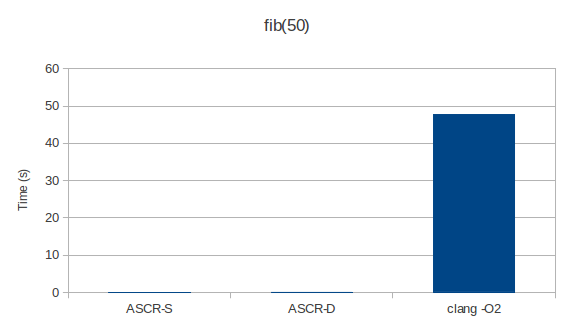
\includegraphics[scale=.5]{../performance.png}
\end{frame}

\begin{frame}
\frametitle{Value (lower is better)}
\centering
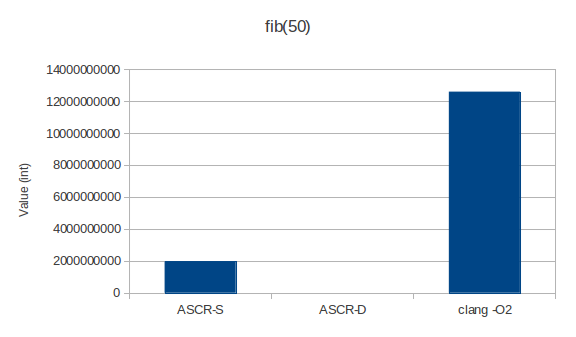
\includegraphics[scale=.5]{../value.png}
\end{frame}

\begin{frame}
\end{frame}

\end{document}

\begin{frame}
\frametitle{Conclusion}
\begin{enumerate}
\item Constrained semantics result in secure, fast programs.
\item Maintain a healthy distrust of your compiler.
\item ASCR decreases your running time and values.
\end{enumerate}
\end{frame}

